\section{Results}\label{sec:results}

\Cref{tab:ratios} compares the bound \eqref{eq:bv-bound} with the empirical loss
\eqref{eq:objective} for several mask ratios, and \cref{fig:curve,fig:sample} show the trend.

\begin{table}[htbp]
  \centering
  \caption{Synthetic numbers: bound versus measured loss.}\label{tab:ratios}
  \begin{tabular}{@{}lccc@{}}
    \toprule
    Ratio $\rho$ & Bound & Measured & Gap $\abs{\Delta}$ \\
    \midrule
    $0.25$ & $0.112$ & $0.118$ & $0.006$ \\
    $0.50$ & $0.254$ & $0.263$ & $0.009$ \\
    $0.75$ & $0.471$ & $0.490$ & $0.019$ \\
    \bottomrule
  \end{tabular}
\end{table}

\begin{figure}[htbp]
  \centering
  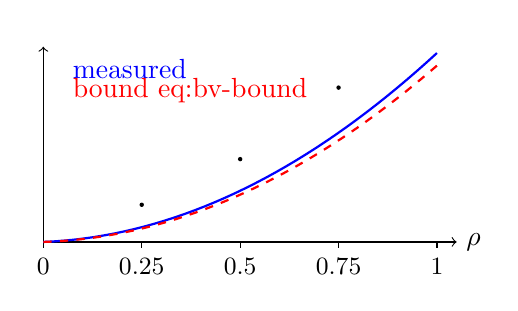
\begin{tikzpicture}[x=5cm, y=4cm]
    \draw[->] (0,0) -- (1.05,0) node[right] {$\rho$};
    \draw[->] (0,0) -- (0,0.62) node[above] {$\loss$};
    \foreach \t in {0,0.25,0.5,0.75,1} \draw (\t,0) -- (\t,-0.02) node[below] {\small $\t$};
    \draw[thick, blue, domain=0:1, samples=40] plot (\x, {0.55*\x*\x + 0.05*\x});
    \draw[thick, red, dashed, domain=0:1, samples=40] plot (\x, {0.52*\x*\x + 0.04*\x});
    \foreach \p/\q in {0.25/0.118, 0.5/0.263, 0.75/0.490} \fill (\p,\q) circle (0.8pt);
    \node[blue, anchor=west] at (0.05,0.55) {measured};
    \node[red, anchor=west] at (0.05,0.48) {bound \eqref{eq:bv-bound}};
  \end{tikzpicture}
  \caption{Loss as a function of the mask ratio (synthetic).}\label{fig:curve}
\end{figure}

\begin{figure}[htbp]
  \centering
  
\includegraphics[width=0.4\linewidth]{figures/heatmap}
  \caption{A synthetic reconstruction error map.}\label{fig:sample}
\end{figure}

\begin{theorem}\label{thm:monotone}
  Under \cref{lem:bias-variance}, the optimal loss is nondecreasing in $\rho$:
  \begin{equation}
    \rho \le \rho' \implies \min_W \Exp\mse[\mask_\rho]{W} \le \min_W \Exp\mse[\mask_{\rho'}]{W}.
    \label{eq:monotone}
  \end{equation}
\end{theorem}

\begin{remark}
  The gap in \cref{tab:ratios} grows roughly like $\rho^2$, consistent with
  \begin{align}
    \Delta(\rho) &\approx c\,\rho^2 + O(\rho^3), \notag \\
    \intertext{and with the fitted constant}
    c &= 0.03 \pm 0.01. \label{eq:fit}
  \end{align}
\end{remark}

\begin{enumerate}[label=(\roman*)]
  \item The bound is tight for linear models (\cref{eq:wstar}).
  \item It is loose by $\epsilon = \oldepsilon/2$ for attention models; see \citep{roe2022views,lee2024note}.
\end{enumerate}
